\documentclass{standalone}
\usepackage{tikz}
\usetikzlibrary{positioning}

\begin{document}
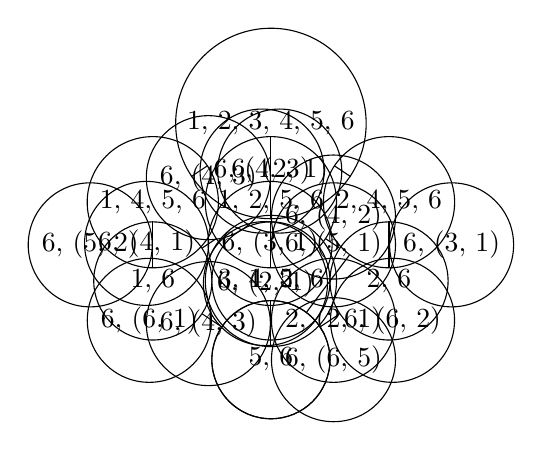
\begin{tikzpicture}[node distance=1cm and 1.5cm, auto, on grid, every node/.style={draw, circle, minimum size=1.5cm}]
    % Nodes
    \node (top) {1, 2, 3, 4, 5, 6};
    \node (n1) [below left=of top] {1, 4, 5, 6};
    \node (n2) [below=of top] {1, 2, 5, 6};
    \node (n3) [below right=of top] {2, 4, 5, 6};
    \node (n4) [below right=of n1] {3, 4, 5, 6};
    \node (n5) [below=of n1] {1, 6};
    \node (n6) [below=of n2] {1, 2};
    \node (n7) [below=of n3] {2, 6};
    \node (n8) [below=of n4] {5, 6};
    \node (bottom) [below=of n6] {};

    % Edges
    \draw (top) -- node[right] {6, (4, 3)} (n1);
    \draw (top) -- node[left] {6, (4, 3)} (n2);
    \draw (top) -- node[left] {6, (2, 1)} (n3);
    \draw (top) -- node[right] {6, (4, 2)} (n4);
    \draw (n1) -- node[left] {6, (5, 2)} (n5);
    \draw (n2) -- node[left] {6, (4, 1)} (n5);
    \draw (n2) -- node[right] {6, (5, 1)} (n6);
    \draw (n2) -- node[left] {6, (3, 1)} (n7);
    \draw (n3) -- node[right] {6, (3, 1)} (n7);
    \draw (n3) -- node[left] {6, (2, 1)} (n8);
    \draw (n4) -- node[left] {6, (4, 3)} (n8);
    \draw (n5) -- node[left] {6, (6, 1)} (bottom);
    \draw (n6) -- node[right] {2, (2, 1)} (bottom);
    \draw (n7) -- node[right] {6, (6, 2)} (bottom);
    \draw (n8) -- node[right] {6, (6, 5)} (bottom);
\end{tikzpicture}
\end{document}